%
% $RCSfile: development_process.tex,v $
%
% Copyright (C) 2002-2008. Christian Heller.
%
% Permission is granted to copy, distribute and/or modify this document
% under the terms of the GNU Free Documentation License, Version 1.1 or
% any later version published by the Free Software Foundation; with no
% Invariant Sections, with no Front-Cover Texts and with no Back-Cover
% Texts. A copy of the license is included in the section entitled
% "GNU Free Documentation License".
%
% http://www.cybop.net
% - Cybernetics Oriented Programming -
%
% http://www.resmedicinae.org
% - Information in Medicine -
%
% Version: $Revision: 1.1 $ $Date: 2008-08-19 20:41:06 $ $Author: christian $
% Authors: Christian Heller <christian.heller@tuxtax.de>
%

\paragraph{A Development Process embedding CYBOP Principles}
\label{development_process_heading}

It would be interesting to know how well the CYBOP principles fit into existing
\emph{Software Engineering Processes} (SEP), like the ones mentioned in chapter
\ref{software_engineering_process_heading}. Probably, an own SEP called
something like \emph{Cybernetics Oriented Methodology} (CYBOM) will have to be
developed for CYBOP.

\begin{figure}[ht]
    \begin{center}
        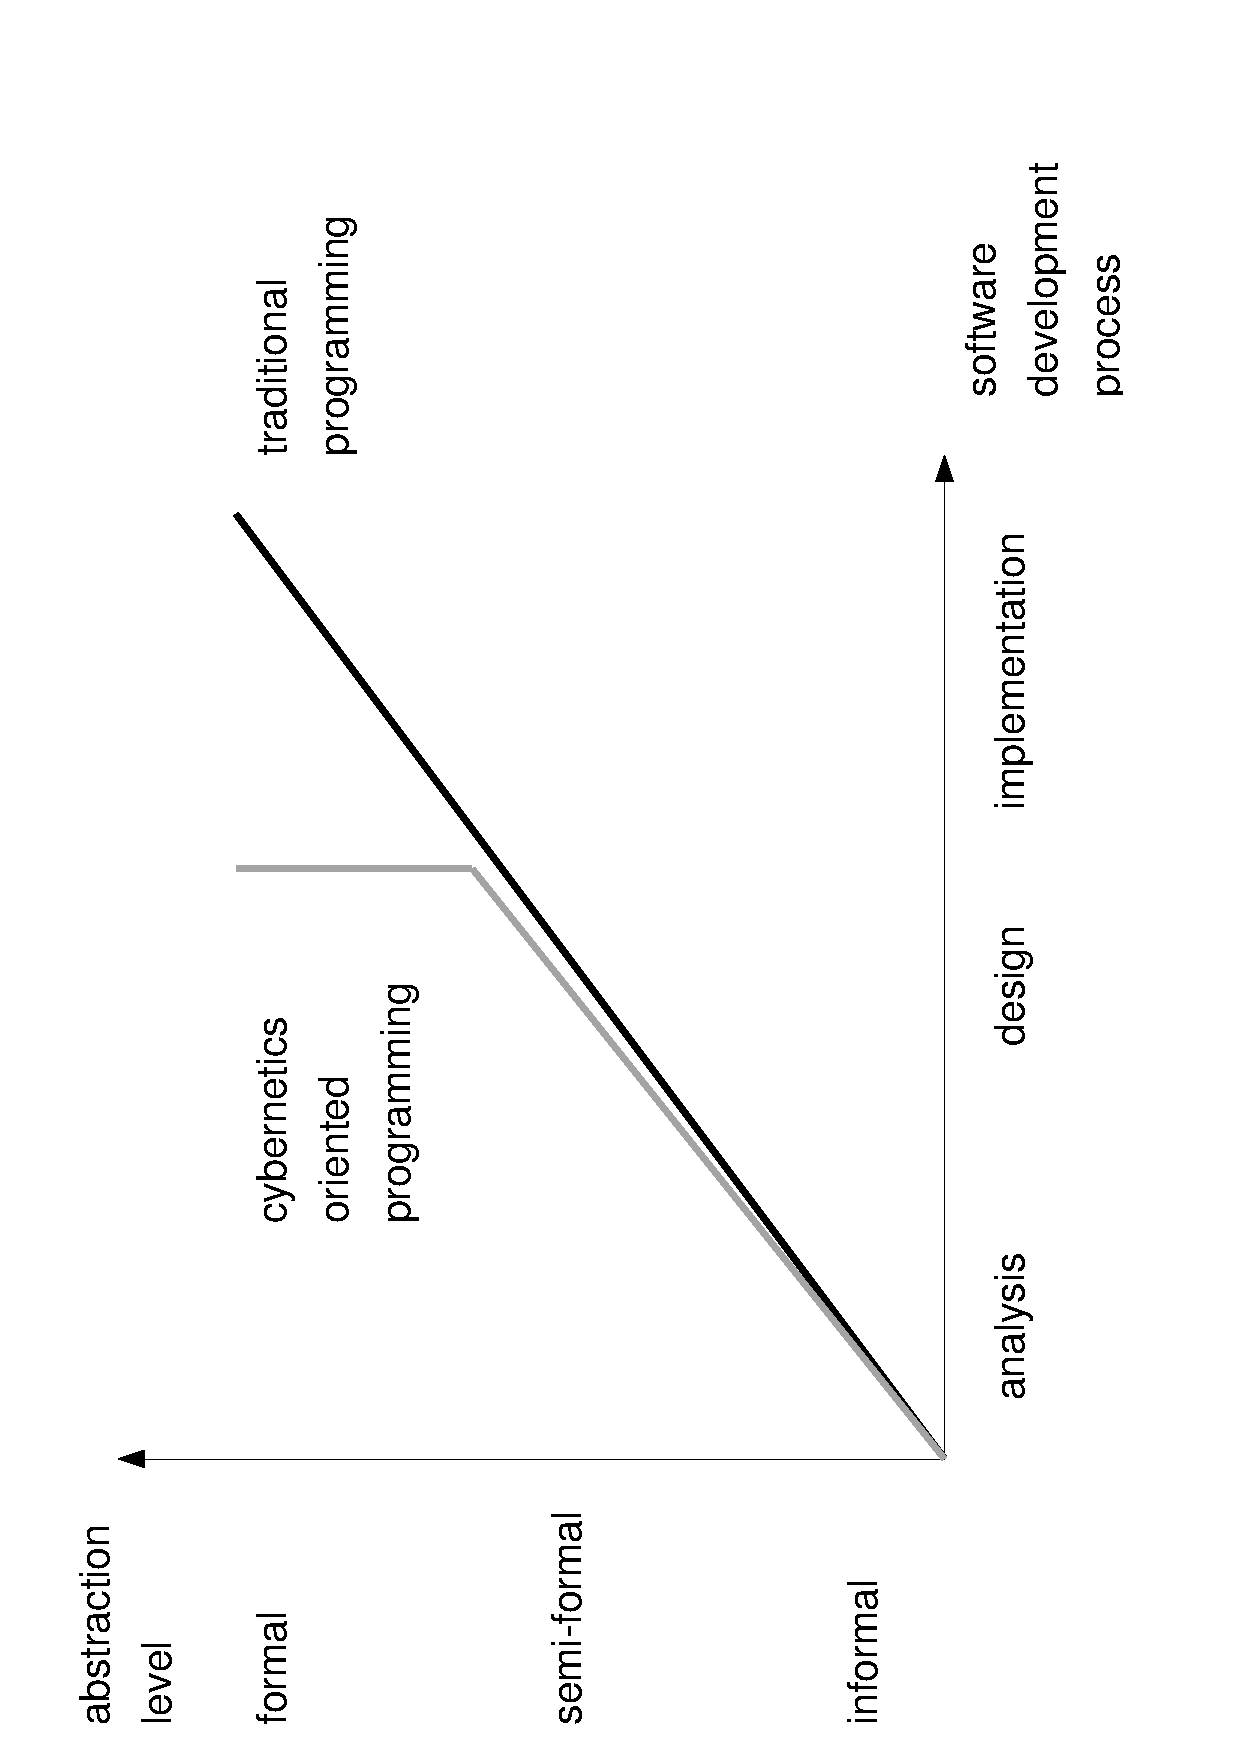
\includegraphics[scale=0.3,angle=-90]{graphic/cybom.pdf}
        \caption{Comparison of a traditional SEP with CYBOM}
        \label{cybom_figure}
    \end{center}
\end{figure}

Of special interest thereby is the missing implementation phase. Figure
\ref{cybom_figure} shows a diagram comparing a traditional- with a
cybernetics-oriented SEP. While the traditional SEP has to pass the three
phases \emph{Analysis}, \emph{Design} and \emph{Implementation}, CYBOM would
stop at the end of the design phase, because its architected knowledge
templates already represent the implementation, specified in a formal language
-- CYBOL.

However, the exact details are still \emph{Speculation}. The figure is
\emph{not} based on research and just a \emph{Guess} how a CYBOM might shorten
the SEP time and effort. Further investigation and proof are needed. Also, it
has to be figured out in how far missing CYBOI features have a delaying
influence, since CYBOL can only make use of functionality that is already
provided by CYBOI.

Strongly related with a CYBOM, is a plan for smoothly \emph{migrating} systems
that have been developed using \emph{Structured- and Procedural Programming}
(SPP) or \emph{Object Oriented Programming} (OOP) techniques, to CYBOP. In
conjunction with it, training methodologies, tutorials etc. are to be created.
